% Document template
\documentclass[a4paper,11pt, hidelinks]{article}

% Image packages
\usepackage{graphicx, pgf, tikz, pgfplots} 

\usepackage{fancyhdr}						% import fancy hdr
\usepackage{msdata}							% import mathscapes data
\usepackage{hyperref}
\usepackage{background}
\usepackage{amsmath}


\SetBgContents{ }

% Set contents
\SetBgColor{black}
\SetBgPosition{current page.west}			% Select location
\SetBgVshift{-1.8cm}
\SetBgOpacity{1}							% Select opacity
\SetBgAngle{90.0}							% Select rotation of logo
\SetBgScale{1.2}							% Select scale factor of logo
\SetBgAnchor{}

% Set date
\usepackage{datetime}						% import datetime package
\newdate{date}{10}{10}{2018}				% set new date
\date{\displaydate{date}}					% configure doc date to new date

% Meta parameters
\setlength{\parindent}{0em}					% remove paragraph indent
\setlength{\parskip}{0.5em}					% set spacing after paragraph
\graphicspath{ {images/} }					% set images path
\fancyhf{}									% clear all header and footers
\renewcommand{\headrulewidth}{0pt}			% remove the header rule
\rfoot{\thepage}					% set page number in right footer


% Copyright message
\chead{}
\lfoot{\mscpy}
\AtEndDocument{\lfoot{}}
\pagestyle{fancy}							% set page styles as fancy


% Document Title
\title{Effect of Fiber Volume Fraction on Composite Response under Ballistic Impact Load}
\author{ 
	Rahul Singh \\
	\small{Mathscapes Research}\\
}

% Document
\begin{document}
\maketitle
\thispagestyle{fancy}

\section{Introduction}
Fiber volume fraction is the ratio which decides on the amount of fiber material and resin presence in the manufacturing of composites. Hence, this ratio plays a significant role in the determining the elastic properties of the material. It is necessary to have the right amount of mix as a minor change in the properties can bring about a catastrophic failure. In the present study, we strive to investigate the variation in the elastic parameters of the material. The study investigates the effect by simulating a ballistic impact load over a lamina with varying fiber volume fraction. The elastic parameters are calculated using the rules of mixture and are then used to determine the response of lamina subjected to ballistic impact. In order to observe the response of lamina, a progressive failure damage model in consideration with a string of failure criteria is implemented while considering fiber and matrix damage that are associated with various modes of failure which occur during the course of damage based on the continuum damage mechanics (CDM) model. A commercial FE code ABAQUS is used to formulate a subroutine VUMAT and simulate the phenomenon of penetration.  The present study investigates the effect of fiber volume fraction on the strength of composite materials. A lamina is subjected to impact by a .22 caliber projectile while varying its volume fraction with help of a Python interface. The damage pattern of lamina are studied to determine the effect of volume fraction.

\section{Damage modeling}
A two dimensional progressive damage model suggested by Matzenmiller et. al.\cite{Matzenmiller1995} is implemented using VUMAT to model the response of composite lamina. The damage model has two phases, namely – damage initiation which occurs when any of failure criteria is satisfied, and damage evolution under which the elastic properties of the lamina deteriorates and ultimately becomes 0 when the material fails. The change in the magnitude of elastic properties results in variation in stresses. The 5 failure modes associated with the composites used are 1 – fiber shear punch, as the fiber tends to distort and in turn giving rise to cracks on the inner surface. Fiber shear punch is a modeified Hashin\cite{Hashin1980} criteria for fiber failure. The criteria are introduced for a unidirectional layer as a quadratic equation –
In axial direction,

\begin{subequations}
    \begin{equation}
        \frac{S_{11}}{F_{1T}}  = {r_1}^2
    \end{equation}

and in the transverse direction,

    \begin{equation}
        \frac{S_{22}}{F_{2T}}  = {r_2}^2
    \end{equation}
\end{subequations}

where, $r_1$ and $r_2$ are the damage thresholds, $F_{1T}$ and $F_{2T}$ are strengths in direction 1 (along the fiber), direction 2 (normal) and $S_{ij}$ are stresses in such that $i = j$ are normal stresses and $i \neq j$ are shear stresses. 2 – fiber failure in compression because of the tendency of fiber to have high compressive stress in the vicinity of point of impact. The compressive fiber failure can be written as –

\begin{subequations}
    \begin{equation}
        \frac{S_{11}}{F_{1C}}  = {r_3}^2
    \end{equation}

    \begin{equation}
        \frac{S_{22}}{F_{2C}}  = {r_4}^2
    \end{equation}
\end{subequations}

where, $r_3$ and $r_4$ are the damage thresholds, $F_{1C}$ and $F_{2C}$ are compressive strengths in direction 1 (along the fiber), direction 2 (normal) and $S_{ij}$ are stresses. 3 – The fibers will end up as a loose bundle upon the failure of matrix material and hence an in-plane matrix criteria in used to identify such instances. Mathematically,

\begin{equation}
    \frac{S_{12}}{F_{12}}  = {r_5}^2
\end{equation}

where, $r_5$ is the damage threshold, $F_{12}$ is shear strength and $S_{12}$ is shear stress. Each failure mode corresponds to a damage variable which in turn records and evaluates the damage evolution by the means of damage growth function given as -

\begin{equation}
    d_j = 1 + \exp^{\frac{1-{r_i}^m}{m}} , r_j > 1
\end{equation}

where $m$ is the material softening parameter that regulates the softening response of laminated composites.  Higher the value of $m$, the laminate will be more brittle in nature and lower values makes it ductile\cite{Gama2009,Xiao2005}. Damage threshold $r_i$ are initially set near to 1, which makes the damage variable 0. But, once the damage initiates, the value of damage thresholds rises until the damage variable reaches to 1.  The value of damage variable 1 causes the elastic parameters of material degrades to 0. The damage variable is employed in stress-strain relation to evaluate the values of stresses. Stresses $[S]$ are computed using the expression\cite{Bandaru2016c}

\begin{equation}
    [S] = [C_d][\epsilon]
\end{equation}

where $[C_d]$ is stiffness matrix that is derived by inverting the compliance matrix $[S_d]$ –

\begin{equation}
    [S_d] =  \begin{bmatrix}\frac{1}{(1-d_1)E_{11}}&\frac{-\nu_{21} }{E_{22}}&0\\\frac{-\nu_{12} }{E_{11}}&\frac{1}{(1-d_2)E_{22}}&0\\0&0&\frac{1}{(1-d_3)G_{12}}\end{bmatrix}
\end{equation}

where $d_j$ are damage variables used to store values of coefficient of stiffness blackuction.

\section{Fiber volume fraction}
The fiber volume fraction is said to have an important role in composite engineering as the material parameters of laminates depends on the composition of fiber and matrix. The ratio is calculated by analyzing the organization of fibers and resins. There are often voids in the material during manufacturing and the same must be accounted for. Too much fiber volume decreases the strength of composite due to the lack of space for matrix to hold it together. And the same can be said if the matrix volume is high which then lacks enough reinforcement. The present study hence investigates the effect of impact response over a range of fiber volume fraction for impact analysis on composites.

There are several methods to calculate the elastic properties of composite lamina using volume fraction. Sudheer M et. al. \cite{Sudheer2015} investigated the variation in the results from rule of mixture, Halpin-Tsai, Nielsen and Chamis elastic models along with analytical and FE pblackicted solutions. Mendoza Jasso et. al.\cite{MendozaJasso2011} studied the effect of volume fraction on failure initiation in a holed plate subjected to tensile loading. You et. al. \cite{You2015} studied the factor influencing the strength of GFRP rebar material and increased it using fiber volume fraction. Young et. al. \cite{You2015} optimized the fiber volume fraction without changing the cross-section of rebars hence enhancing the tensile properties. The spaces between fibres were removed by filling it and making a compact core by tightly surface wrapping them. Other previous works\cite{Zheng2017, Sudheer2015} used various mathematical expressions to pblackict the elastic constants such as stiffness and strength of composite material. Rule of mixture is applied in the present study to investigate the effect of volume fraction.

Longitudinal properties \cite{Sudheer2015} ,

\begin{subequations}
    \begin{equation}
        E_1 = V_f E_f + ( 1 - V_f) (E_m)
    \end{equation}

    \begin{equation}
        \nu _1 = V_f \nu_f + ( 1 - V_f) (\nu_m)
    \end{equation}
\end{subequations}

Transverse properties \cite{Sudheer2015} ,

\begin{subequations}
	\begin{equation}
		\frac {E_{11}E_m}{V_f E_f + V_m E_m}
	\end{equation}
	
	\begin{equation}
		\frac {\nu_{12}E_2}{E_1}
	\end{equation}
\end{subequations}


Shear properties

\begin{equation}
    \frac {G_{12}}{V_f G_f + V_m G_m}
\end{equation}

where,  Young’s modulus of the matrix and fiber are taken as $E_m$ and $E_f$. Poisson’s ratio are taken as $\nu_m$ and $\nu_f$ respectively. Elastic properties of lamina are $E_{11}$, $E_{22}$ and $G_{12}$.

\section{Results and Discussion}
Initially while implementing the work of Sudheer M. et. al. \cite{Sudheer2015}, change in Young’s modulus and Shear modulus is obtained with variation in fiber volume fraction. The Young’s modulus, $E_1$ is plotted in Fig. 1. It can be observed that the E1 varies linearly with respect to change in volume fraction. Similar observation can be made for Poison ratio $P_{12}$ and $P_{21}$ are plotted in Fig. 1.

\begin{figure}[h]
  \centering
  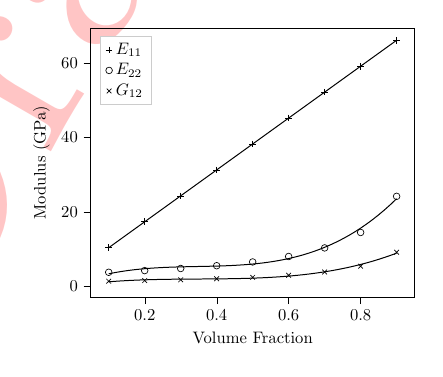
\begin{tikzpicture}[scale=0.6]
\begin{axis}[
legend cell align={left},
legend style={at={(0.03,0.97)}, anchor=north west, draw=white!80.0!black},
tick align=outside,
tick pos=left,
x grid style={white!69.01960784313725!black},
xlabel={ Volume Fraction},
xmin=0.0501433691756272, xmax=0.949856630824373,
xtick style={color=black},
y grid style={white!69.01960784313725!black},
ylabel={ Modulus (GPa) },
ymin=-2.82809617775432, ymax=69.4334108660278,
ytick style={color=black}
]
\addplot [only marks, mark=+, draw=black, fill=black]
table{%
x                      y
0.1 10.415
0.2 17.38
0.3 24.345
0.4 31.31
0.5 38.275
0.6 45.24
0.7 52.205
0.8 59.17
0.9 66.135
};
\addlegendentry{$E_{11}$}
\addplot [only marks, mark=o, draw=black!50.0!black, colormap/viridis]
table{%
x                      y
0.1 3.81333635745067
0.2 4.26221057968565
0.3 4.83085911311177
0.4 5.57460212201592
0.5 6.58902677988243
0.6 8.05477483232194
0.7 10.3592113370302
0.8 14.5106444188723
0.9 24.2145943350936
};
\addlegendentry{$E_{22}$}
\addplot [only marks, mark=x, draw=black, fill=black, colormap/viridis]
table{%
x                      y
0.1 1.41539845565635
0.2 1.58283031522468
0.3 1.7951887420367
0.4 2.07335822534593
0.5 2.4535412605588
0.6 3.004455760662
0.7 3.87441001436487
0.8 5.45349508954362
0.9 9.20526572403706
};
\addlegendentry{$G_{12}$}
\addplot [semithick, black, forget plot]
table {%
0.1 10.415
0.116326530612245 11.5521428571429
0.13265306122449 12.6892857142857
0.148979591836735 13.8264285714286
0.16530612244898 14.9635714285714
0.181632653061225 16.1007142857143
0.197959183673469 17.2378571428571
0.214285714285714 18.375
0.230612244897959 19.5121428571428
0.246938775510204 20.6492857142857
0.263265306122449 21.7864285714286
0.279591836734694 22.9235714285714
0.295918367346939 24.0607142857143
0.312244897959184 25.1978571428571
0.328571428571429 26.335
0.344897959183673 27.4721428571428
0.361224489795918 28.6092857142857
0.377551020408163 29.7464285714285
0.393877551020408 30.8835714285714
0.410204081632653 32.0207142857143
0.426530612244898 33.1578571428571
0.442857142857143 34.295
0.459183673469388 35.4321428571428
0.475510204081633 36.5692857142857
0.491836734693878 37.7064285714286
0.508163265306122 38.8435714285714
0.524489795918367 39.9807142857143
0.540816326530612 41.1178571428571
0.557142857142857 42.255
0.573469387755102 43.3921428571429
0.589795918367347 44.5292857142857
0.606122448979592 45.6664285714286
0.622448979591837 46.8035714285714
0.638775510204082 47.9407142857143
0.655102040816327 49.0778571428571
0.671428571428571 50.215
0.687755102040816 51.3521428571429
0.704081632653061 52.4892857142857
0.720408163265306 53.6264285714286
0.736734693877551 54.7635714285715
0.753061224489796 55.9007142857143
0.769387755102041 57.0378571428572
0.785714285714286 58.175
0.802040816326531 59.3121428571429
0.818367346938776 60.4492857142857
0.83469387755102 61.5864285714286
0.851020408163265 62.7235714285715
0.86734693877551 63.8607142857143
0.883673469387755 64.9978571428572
0.9 66.135
};
\addplot [semithick, black!50.0!black, forget plot]
table {%
0.1 3.40478775360321
0.116326530612245 3.7139180541356
0.13265306122449 3.98610530679498
0.148979591836735 4.22398019593995
0.16530612244898 4.43017340592909
0.181632653061225 4.607315621121
0.197959183673469 4.75803752587427
0.214285714285714 4.8849698045475
0.230612244897959 4.99074314149927
0.246938775510204 5.07798822108819
0.263265306122449 5.14933572767283
0.279591836734694 5.20741634561181
0.295918367346939 5.2548607592637
0.312244897959184 5.2942996529871
0.328571428571429 5.32836371114061
0.344897959183673 5.35968361808281
0.361224489795918 5.39089005817231
0.377551020408163 5.42461371576769
0.393877551020408 5.46348527522754
0.410204081632653 5.51013542091046
0.426530612244898 5.56719483717504
0.442857142857143 5.63729420837987
0.459183673469388 5.72306421888356
0.475510204081633 5.82713555304468
0.491836734693878 5.95213889522183
0.508163265306122 6.10070492977361
0.524489795918367 6.2754643410586
0.540816326530612 6.47904781343541
0.557142857142857 6.71408603126262
0.573469387755102 6.98320967889882
0.589795918367347 7.28904944070261
0.606122448979592 7.63423600103259
0.622448979591837 8.02140004424733
0.638775510204082 8.45317225470545
0.655102040816327 8.93218331676552
0.671428571428571 9.46106391478615
0.687755102040816 10.0424447331259
0.704081632653061 10.6789564561434
0.720408163265306 11.3732297681973
0.736734693877551 12.127895353646
0.753061224489796 12.9455838968483
0.769387755102041 13.8289260821627
0.785714285714286 14.7805525939478
0.802040816326531 15.8030941165622
0.818367346938776 16.8991813343645
0.83469387755102 18.0714449317132
0.851020408163265 19.3225155929671
0.86734693877551 20.6550240024845
0.883673469387755 22.0716008446243
0.9 23.5748768037449
};
\addplot [semithick, black, forget plot]
table {%
0.1 1.25517122006906
0.116326530612245 1.37494422124114
0.13265306122449 1.48024219511787
0.148979591836735 1.57208836648409
0.16530612244898 1.65150596012466
0.181632653061225 1.71951820082443
0.197959183673469 1.77714831336825
0.214285714285714 1.82541952254099
0.230612244897959 1.86535505312749
0.246938775510204 1.89797812991262
0.263265306122449 1.92431197768121
0.279591836734694 1.94537982121814
0.295918367346939 1.96220488530825
0.312244897959184 1.9758103947364
0.328571428571429 1.98721957428744
0.344897959183673 1.99745564874622
0.361224489795918 2.00754184289761
0.377551020408163 2.01850138152645
0.393877551020408 2.03135748941761
0.410204081632653 2.04713339135592
0.426530612244898 2.06685231212626
0.442857142857143 2.09153747651347
0.459183673469388 2.1222121093024
0.475510204081633 2.15989943527792
0.491836734693878 2.20562267922488
0.508163265306122 2.26040506592812
0.524489795918367 2.32526982017252
0.540816326530612 2.40124016674291
0.557142857142857 2.48933933042415
0.573469387755102 2.59059053600111
0.589795918367347 2.70601700825862
0.606122448979592 2.83664197198156
0.622448979591837 2.98348865195476
0.638775510204082 3.1475802729631
0.655102040816327 3.32994005979141
0.671428571428571 3.53159123722456
0.687755102040816 3.7535570300474
0.704081632653061 3.99686066304478
0.720408163265306 4.26252536100156
0.736734693877551 4.55157434870259
0.753061224489796 4.86503085093273
0.769387755102041 5.20391809247683
0.785714285714286 5.56925929811975
0.802040816326531 5.96207769264634
0.818367346938776 6.38339650084145
0.83469387755102 6.83423894748994
0.851020408163265 7.31562825737668
0.86734693877551 7.82858765528649
0.883673469387755 8.37414036600425
0.9 8.9533096143148
};
\end{axis}
\end{tikzpicture}
%
\hskip 5pt
%
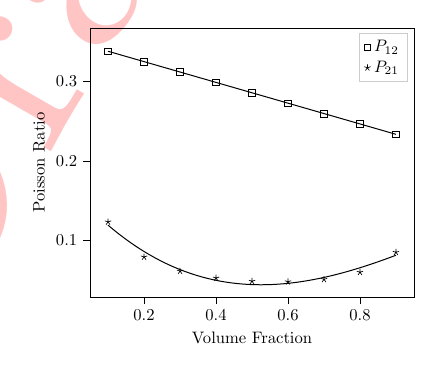
\begin{tikzpicture}[scale=0.6]
\begin{axis}[
legend cell align={left},
legend style={draw=white!80.0!black},
tick align=outside,
tick pos=left,
x grid style={white!69.01960784313725!black},
xlabel={ Volume Fraction},
xmin=0.0501433691756272, xmax=0.949856630824373,
xtick style={color=black},
y grid style={white!69.01960784313725!black},
ylabel={ Poisson Ratio },
ymin=0.0293324378717648, ymax=0.366104741474203,
ytick style={color=black}
]
\addplot [only marks, mark=square, draw=black, colormap/viridis]
table{%
x                      y
0.1 0.337
0.2 0.324
0.3 0.311
0.4 0.298
0.5 0.285
0.6 0.272
0.7 0.259
0.8 0.246
0.9 0.233
};
\addlegendentry{$P_{12}$}
\addplot [only marks, mark=star, draw=black, colormap/viridis]
table{%
x                      y
0.1 0.123388800044251
0.2 0.0794566299089845
0.3 0.0617127617242868
0.4 0.0530575353676379
0.5 0.04906264225386
0.6 0.0484283544295218
0.7 0.051394229217332
0.8 0.0603281819679327
0.9 0.0853103573006247
};
\addlegendentry{$P_{21}$}
\addplot [semithick, black, forget plot]
table {%
0.1 0.337
0.116326530612245 0.334877551020408
0.13265306122449 0.332755102040816
0.148979591836735 0.330632653061225
0.16530612244898 0.328510204081633
0.181632653061225 0.326387755102041
0.197959183673469 0.324265306122449
0.214285714285714 0.322142857142857
0.230612244897959 0.320020408163265
0.246938775510204 0.317897959183674
0.263265306122449 0.315775510204082
0.279591836734694 0.31365306122449
0.295918367346939 0.311530612244898
0.312244897959184 0.309408163265306
0.328571428571429 0.307285714285714
0.344897959183673 0.305163265306123
0.361224489795918 0.303040816326531
0.377551020408163 0.300918367346939
0.393877551020408 0.298795918367347
0.410204081632653 0.296673469387755
0.426530612244898 0.294551020408163
0.442857142857143 0.292428571428572
0.459183673469388 0.29030612244898
0.475510204081633 0.288183673469388
0.491836734693878 0.286061224489796
0.508163265306122 0.283938775510204
0.524489795918367 0.281816326530612
0.540816326530612 0.279693877551021
0.557142857142857 0.277571428571429
0.573469387755102 0.275448979591837
0.589795918367347 0.273326530612245
0.606122448979592 0.271204081632653
0.622448979591837 0.269081632653061
0.638775510204082 0.266959183673469
0.655102040816327 0.264836734693878
0.671428571428571 0.262714285714286
0.687755102040816 0.260591836734694
0.704081632653061 0.258469387755102
0.720408163265306 0.25634693877551
0.736734693877551 0.254224489795918
0.753061224489796 0.252102040816327
0.769387755102041 0.249979591836735
0.785714285714286 0.247857142857143
0.802040816326531 0.245734693877551
0.818367346938776 0.243612244897959
0.83469387755102 0.241489795918367
0.851020408163265 0.239367346938776
0.86734693877551 0.237244897959184
0.883673469387755 0.235122448979592
0.9 0.233
};
\addplot [semithick, black, forget plot]
table {%
0.1 0.119270310115613
0.116326530612245 0.113133032272472
0.13265306122449 0.107296386621284
0.148979591836735 0.101755463054848
0.16530612244898 0.0965053514659615
0.181632653061225 0.0915411417474224
0.197959183673469 0.0868579237920288
0.214285714285714 0.0824507874925788
0.230612244897959 0.0783148227418704
0.246938775510204 0.0744451194327017
0.263265306122449 0.0708367674578707
0.279591836734694 0.0674848567101754
0.295918367346939 0.0643844770824139
0.312244897959184 0.0615307184673841
0.328571428571429 0.0589186707578841
0.344897959183673 0.056543423846712
0.361224489795918 0.0544000676266658
0.377551020408163 0.0524836919905435
0.393877551020408 0.0507893868311431
0.410204081632653 0.0493122420412627
0.426530612244898 0.0480473475137003
0.442857142857143 0.0469897931412539
0.459183673469388 0.0461346688167216
0.475510204081633 0.0454770644329014
0.491836734693878 0.0450120698825914
0.508163265306122 0.0447347750585895
0.524489795918367 0.0446402698536938
0.540816326530612 0.0447236441607023
0.557142857142857 0.0449799878724132
0.573469387755102 0.0454043908816242
0.589795918367347 0.0459919430811337
0.606122448979592 0.0467377343637395
0.622448979591837 0.0476368546222397
0.638775510204082 0.0486843937494323
0.655102040816327 0.0498754416381153
0.671428571428571 0.0512050881810869
0.687755102040816 0.052668423271145
0.704081632653061 0.0542605368010876
0.720408163265306 0.0559765186637129
0.736734693877551 0.0578114587518186
0.753061224489796 0.0597604469582031
0.769387755102041 0.0618185731756643
0.785714285714286 0.0639809272970002
0.802040816326531 0.0662425992150088
0.818367346938776 0.0685986788224882
0.83469387755102 0.0710442560122365
0.851020408163265 0.0735744206770515
0.86734693877551 0.0761842627097314
0.883673469387755 0.0788688720030742
0.9 0.0816233384498781
};
\end{axis}

\end{tikzpicture}

  \caption{Variation in modulus $E_1$, $E_2$ and $G_{12}$ with respect to volume fraction}
\end{figure}


All analysis were executed by considering a target lamina of diameter 25.4 * 254 mm and width 0.272 mm. A .22 caliber projectile of diameter .22 inch with a rigid mass of 3.14 g is impacted on the target with varying volume fraction of composite plates from 0.1 to 0.9 and at velocity 100 m/s. The plate is fixed on both sides, and the projectile is moving in the z-direction. It is discretized using eight node linear brick element with blackuced integration (C3D8R) whereas, R3D4 is used for the projectile, both having mesh size of 0.2 mm x 0.2 mm. A total of 40005 and 840 elements are generated in disc and projectile respectively. A general contact algorithm is used to formulate contact between disc and projectile with a penalty contact of friction coefficient 0.3. It is observed that the volume fraction of 0.5 and 0.75 absorbs the most energy.
	
It is observed that volume fraction 0.5 and 0.75 exhibits more elastic response to the projectile and hence are able to absorb relatively more energy. The laminae with volume fraction 0.5 and 0.75 have more elastic response and hence more deflection.

It is observed that though the magnitude of moduli is increasing but as the fiber volume fraction increases, it makes the lamina act like a loose bundle of fibers and hence not able to absorb enough energy from projectile. The volume fraction in the range 0.5 to 0.75 is resulting in the lower value of residual velocity which means the lamina of volume fraction 0.5 to 0.75 are absorbing more energy than the rest and hence is the range from which the values of 0.5 to 0.75.

\begin{figure}[h]
  \centering
  
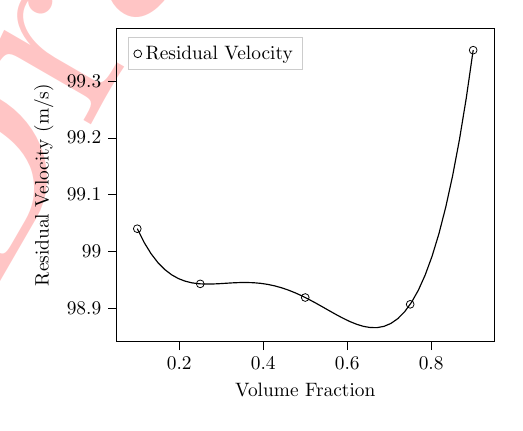
\begin{tikzpicture}[scale=0.7]

\begin{axis}[
legend cell align={left},
legend style={at={(0.03,0.97)}, anchor=north west, draw=white!80.0!black},
tick align=outside,
tick pos=left,
x grid style={white!69.01960784313725!black},
xlabel={ Volume Fraction},
xmin=0.0501433691756272, xmax=0.949856630824373,
xtick style={color=black},
y grid style={white!69.01960784313725!black},
ylabel={ Residual Velocity (m/s) },
ymin=98.8409653507578, ymax=99.3928841265749,
ytick style={color=black}
]
\addplot [only marks, mark=o, draw=black, fill=black, colormap/viridis]
table{%
x                      y
0.1 99.04
0.25 98.943
0.5 98.919
0.75 98.907
0.9 99.354
};
\addlegendentry{Residual Velocity}
\addplot [semithick, black, forget plot]
table {%
0.1 99.0400000000001
0.116326530612245 99.015854825377
0.13265306122449 98.9962062667505
0.148979591836735 98.9805184075971
0.16530612244898 98.9682840407288
0.181632653061225 98.959024668293
0.197959183673469 98.9522905017729
0.214285714285714 98.947660461987
0.230612244897959 98.9447421790895
0.246938775510204 98.9431719925699
0.263265306122449 98.9426149512534
0.279591836734694 98.9427648133006
0.295918367346939 98.9433440462079
0.312244897959184 98.9441038268069
0.328571428571429 98.9448240412649
0.344897959183673 98.9453132850847
0.361224489795918 98.9454088631046
0.377551020408163 98.9449767894984
0.393877551020408 98.9439117877756
0.410204081632653 98.9421372907809
0.426530612244898 98.9396054406949
0.442857142857143 98.9362970890335
0.459183673469388 98.9322217966481
0.475510204081633 98.9274178337258
0.491836734693878 98.9219521797891
0.508163265306122 98.915920523696
0.524489795918367 98.9094472636402
0.540816326530612 98.9026855071507
0.557142857142857 98.8958170710923
0.573469387755102 98.8890524816649
0.589795918367347 98.8826309744044
0.606122448979592 98.8768204941819
0.622448979591837 98.8719176952043
0.638775510204082 98.8682479410137
0.655102040816327 98.866165304488
0.671428571428571 98.8660525678404
0.687755102040816 98.8683212226199
0.704081632653061 98.8734114697108
0.720408163265306 98.8817922193331
0.736734693877551 98.8939610910421
0.753061224489796 98.9104444137288
0.769387755102041 98.9317972256197
0.785714285714286 98.9586032742768
0.802040816326531 98.9914750165977
0.818367346938776 99.0310536188154
0.83469387755102 99.0780089564985
0.851020408163265 99.1330396145511
0.86734693877551 99.1968728872128
0.883673469387755 99.2702647780589
0.9 99.3540000000001
};
\end{axis}

\end{tikzpicture}

  \caption{Variation in residual velocity due to change in volume fraction}
\end{figure}

\section{Conclusion}
The effect of fiber volume fraction in behaviour of composite lamina subjected to ballistic impact loading is investigated in present work. The conjunction of Python, ABAQUS and FORTRAN is addressed to perform automation. An interface, developed using Python, is capable to interact with ABAQUS, to modify the material parameters. The material parameters are calculated using the rule of mixture by numpy module in Python and are then forwarded to ABAQUS Material library where it gets modified. The ABAQUS then runs the analysis for that particular set of material parameters and returns again to fetch the new set of parameters. The results shows there is a variation in behaviour of lamina with different volume fractions.
The variation in fiber volume fraction is calculated using the rule of mixture formula a
nd fed into the python interface.

\begin{itemize}
    \item The residual velocity is plotted to study the response of lamina.
    \item The lamina with fiber volume fraction of around 0.1 is said to have a low amount of fibers but high matrix material resulting in less absorption of energy.
    \item The lamina with fiber volume fraction of 0.9 acts like a loose bundle of fibers due to inability of matrix to hold it together.
    \item The lamina with fiber volume fraction of 0.5 to 0.75 is shown to have the maximum absorption of energy. Hence, the ideal value of fiber volume fraction lies in the region which is also in agreement with suggestion from Gibson et. al.\cite{Gibson1994}.
\end{itemize}

% Don't edit this
% ===============
\bibliographystyle{unsrt}
\bibliography{bibiliography.bib}
% ===============

\vspace*{\fill}
\rule{\textwidth}{0.4pt}
\footnotesize \textbf{Usage and permission.} This paper or any portion thereof may not be reproduced or used in any manner whatsoever without the express written permission of Mathscapes Research except for the use of brief quotations in a review.
\end{document}
